\chapter{The System Dependence Graph} \label{ch:sdg}

As mentioned before, a system dependence graph (SDG) is a way to represent a program in its entirety as far as control 
and data dependencies are concerned. Note however that the control flow itself is not encoded in the SDG. Consider, for 
example, two statements in a procedure, which are control dependent on that procedure (meaning they will be executed 
whenever the procedure is executed). The SDG does not contain any information about the order in which those two 
statements will be executed when the procedure is called, this information is only available in the control flow graph.

The CSDG used here, in addition to control and data dependencies, also encodes variability in the form of conditions on 
edges. Those so-called presence conditions are Boolean expressions that encode for which combinations of enabled 
features an edge is present in the graph. A feature in this context is, for example, a configuration option that's read 
from a global variable. Since these conditions are of no concern to the visualization and exploration of the SDG 
itself, I will ignore them most of the time. They may however be useful in future additions to the \SB.

The following two sections will describe the implementation and construction of the SDG, and give a detailed 
explanation of its structural properties.


\section{Structure}

\Todo{Explain structure in detail}


\section{Construction and Implementation}

The construction of the SDG is covered in great detail in Andreas Grimmer's master thesis~\cite{GrimmerDA}, the 
following section will only give a brief overview.

The input for the SDG construction is a PLC program written in the IEC 61131-3 family of 
languages~\cite{IEC61131:2003}, specifically a proprietary dialect of the language used by KEBA. The program is first 
parsed into an abstract syntax tree (AST) which is based on the OMG ASTM~\cite{ASTM} and was extended to handle 
language-specific features~\cite[ch.~4]{GrimmerDA}. 

The ASTM representation is then used to generate Jimple code, an intermediate language representation used by the Soot 
analysis framework~\cite{Soot}. Soot is used to perform control flow and points-to analyses, and it provides def-use 
information and post-dominator trees used in the construction of the SDG.

The SDG is then created in two steps~\cite[ch.~6]{GrimmerDA}.

\begin{enumerate}
  \item In the first step, a program dependence graph (PDG) is built for each procedure in the program. The nodes in 
  this graph represent statements and formal parameters, the edges represent the intra-procedural control and data 
  dependencies between nodes. The PDGs are object-insensitive, which means they are computed once for each procedure 
  rather than based on object instances.
  
  \item From the PDGs the object-sensitive SDG is created by instantiating each PDG according to the object instances 
  it is used in. Information about object instances is provided by Soot's points-to analysis. The PDGs are linked by 
  introducing control edges that link calls to called procedures, and data edges between actual and formal parameter 
  nodes. Since a PLC program may have several entry points, an artificial procedure node is created for the 
  \lstinline|main| procedure, which links to all actual entry points into the program.
\end{enumerate}

\subsection{SDG Classes}

The SDG is represented by classes \lstinline|DGNode| and \lstinline|DGEdge|, which are the abstract base classes for 
different kinds of nodes and edges, and by the class \lstinline|SystemDependenceGraph| which specifies the main entry 
point. \autoref{fig:sdg-class} shows a class diagram of all SDG classes.

\begin{itemize}
  \item Each node has a list of successors and predecessors, edges which link to and from other nodes, respectively.
  
  \item A node may have a seed condition associated with it, a Boolean expression that specifies for what feature 
  combinations dependent nodes are reachable.
  
  \item A \lstinline|PDGNode| represents a statement in the program, whether it be conditional or not.
  
  \item There are three subclasses of \lstinline|SDGNode|, which represent procedure instances and their interactions. 
  Each \lstinline|SDGNode| has an owning \lstinline|Procedure| associated with it, which represents an instance of a 
  procedure much like a \lstinline|ProcedureNode|.
  \begin{itemize}
    \item A \lstinline|ProcedureNode| represents an instance of a procedure and may have zero or more formal parameter 
    nodes associated with it.
    
    \item \lstinline|ExprNode| may represent formal or actual parameters, as well as global variables. In the case of a 
    formal parameter node for a global variable accessed by a procedure, the node also refers to the actual node 
    representing the global variable itself.
    
    \item Calls between procedures are represented by \lstinline|ActivationNode|s. An activation node refers to the 
    statement that represents the call, has one or more procedures that are called (more than one procedure may be 
    called, e.g. by setting an event), and has all actual parameters for the call attached to it.
  \end{itemize}
  
  \item An edge may have a presence condition associated with it, a Boolean expression that specifies for what feature 
  combinations the edge does exist.
  
  \item A \lstinline|ControlEdge| has an associated label, which in the case of conditional statements specifies 
  whether the control dependency is for the true or false branch of the condition.
\end{itemize}

\begin{figure}[hpb]
  \centering
    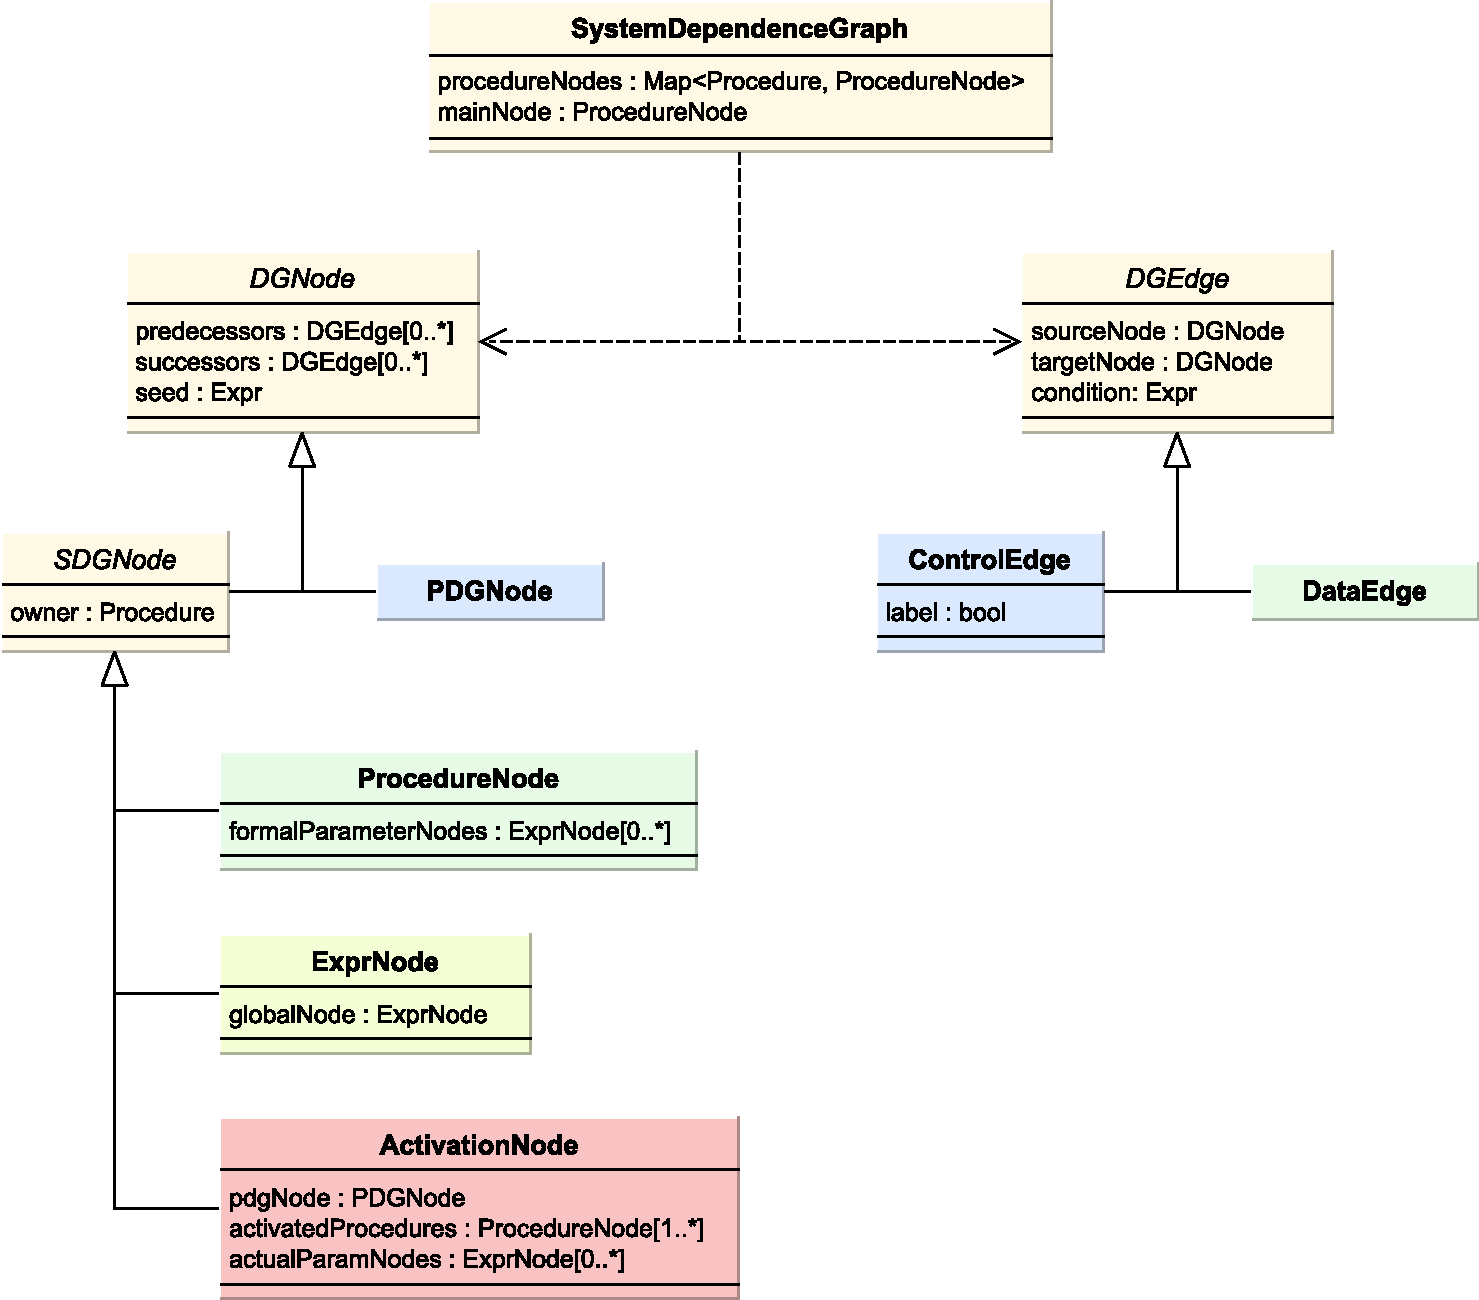
\includegraphics[width=\textwidth]{bilder/sdg-class}
  \caption{Class diagram of the SDG classes}
  \label{fig:sdg-class}
\end{figure}
